\documentclass[11pt,letterpaper]{article}
\usepackage[margin=1in]{geometry}
\usepackage{graphicx}
\usepackage{amsmath}
\usepackage{enumitem}
\usepackage{xcolor}
\usepackage[colorlinks=true,linkcolor=blue,urlcolor=blue]{hyperref}
\usepackage[most]{tcolorbox}
\usepackage{titlesec}
\usepackage{parskip}

\definecolor{accent}{HTML}{2c3e50}

\titleformat{\section}{\large\bfseries\color{accent}}{\thesection}{1em}{}

\setlength{\parindent}{0pt}

\title{\color{accent}Homework}
\author{}
\date{Modules 1--8 \quad·\quad ${\sim}$2.5 hours \quad·\quad Open the interactive tutorial while you work}

\begin{document}
\maketitle
\thispagestyle{empty}

\begin{tcolorbox}[colback=accent!5,colframe=accent,boxrule=0.6pt,arc=4pt,
  left=10pt,right=10pt,top=8pt,bottom=8pt]
Open the tutorial in your browser before starting. Every answer can be found by
reading the modules and playing with the interactive widgets. Show your work
where math is involved. Write your answer in the space provided.
\textbf{Estimated time: 2 hours.}
\end{tcolorbox}

\vspace{1em}

% ──────────────────────────────────────────────────────────────────────
\section*{Problem 1 — Signals}
A patient's alpha rhythm has frequency 10\,Hz and amplitude 30\,$\mu$V.
\begin{enumerate}[label=(\alph*),leftmargin=*]
\item What is its period in milliseconds?
\item How many full cycles fit in one second?
\end{enumerate}

\vspace{3.5cm}
\hfill\textit{\small refer to: \href{https://judepj.github.io/neuro-signals-101/modules/01_signals.html}{Module 1 — Signals}}

\vfill\pagebreak

% ──────────────────────────────────────────────────────────────────────
\section*{Problem 2 — Sampling}
An EEG amplifier samples at 256\,Hz.
\begin{enumerate}[label=(\alph*),leftmargin=*]
\item What is the highest signal frequency you can faithfully record?
\item If a 200\,Hz EMG burst contaminates the recording, at what frequency does it appear in the digitized signal?
\end{enumerate}

\vspace{4cm}
\hfill\textit{\small refer to: \href{https://judepj.github.io/neuro-signals-101/modules/02_sampling.html}{Module 2 — Sampling}}

\vfill

% ──────────────────────────────────────────────────────────────────────
\section*{Problem 3 — Filtering}
\begin{enumerate}[label=(\alph*),leftmargin=*]
\item European mains electrical noise sits at 50\,Hz. What type of filter would you use to remove it?
\item If you set the low-pass filter too aggressively (e.g., cut everything above 15\,Hz), what important EEG feature might you miss, and why is that clinically dangerous?
\end{enumerate}

\vspace{4cm}
\hfill\textit{\small refer to: \href{https://judepj.github.io/neuro-signals-101/modules/03_filtering.html}{Module 3 — Filtering}}

\vfill\pagebreak

% ──────────────────────────────────────────────────────────────────────
\section*{Problem 4 — FFT}
You record a 4-second EEG segment sampled at 250\,Hz.
\begin{enumerate}[label=(\alph*),leftmargin=*]
\item How many samples is that?
\item What is the frequency resolution of an FFT of the whole segment?
\item If you instead split the recording into 1-second windows and FFT each, what does the resolution become?
\end{enumerate}

\vspace{4.5cm}
\hfill\textit{\small refer to: \href{https://judepj.github.io/neuro-signals-101/modules/04_fft.html}{Module 4 — FFT}}

\vfill

% ──────────────────────────────────────────────────────────────────────
\section*{Problem 5 — EEG Frequency Bands}
Match each brain state to its dominant EEG rhythm and state the approximate
frequency band. (Hint: try the clinical-scenario presets in the Band Builder.)

\vspace{0.6em}
\begin{tabular}{p{4.5cm}p{4cm}p{4.5cm}}
\textbf{Brain state} & \textbf{Rhythm name} & \textbf{Frequency band (Hz)} \\
\hline
\rule{0pt}{1.3em} Deep sleep (N3) &  &  \\[1.3em]
Drowsy &  &  \\[1.3em]
Awake, eyes closed &  &  \\[1.3em]
Focused mental task &  &  \\[1.3em]
Active thinking / cognition &  &  \\[1.3em]
\hline
\end{tabular}

\vspace{2.5cm}
\hfill\textit{\small refer to: \href{https://judepj.github.io/neuro-signals-101/modules/05_eeg_basics.html}{Module 5 — EEG Basics}}

\vfill\pagebreak

% ──────────────────────────────────────────────────────────────────────
\section*{Problem 6 — The 10-20 Electrode Naming System}
Each EEG electrode has a name with a letter and a number. For each electrode
below, name the brain region it sits over and which side of the head it is on
(left, right, or midline).

\vspace{0.4em}
\begin{tabular}{p{2.2cm}p{6cm}p{4cm}}
\textbf{Electrode} & \textbf{Brain region} & \textbf{Side} \\
\hline
\rule{0pt}{1.3em} Fp2 &  &  \\[1.2em]
T3 &  &  \\[1.2em]
Pz &  &  \\[1.2em]
O1 &  &  \\[1.2em]
\hline
\end{tabular}

\vspace{3cm}
\hfill\textit{\small refer to: \href{https://judepj.github.io/neuro-signals-101/modules/05_eeg_basics.html}{Module 5 — EEG Basics (10-20 System)}}

\vfill\pagebreak

% ──────────────────────────────────────────────────────────────────────
\section*{Problem 7 — Phase Reversal}
Look at the four-channel bipolar EEG trace below. The display follows clinical
convention (\emph{negative voltage deflects upward}).

\begin{center}
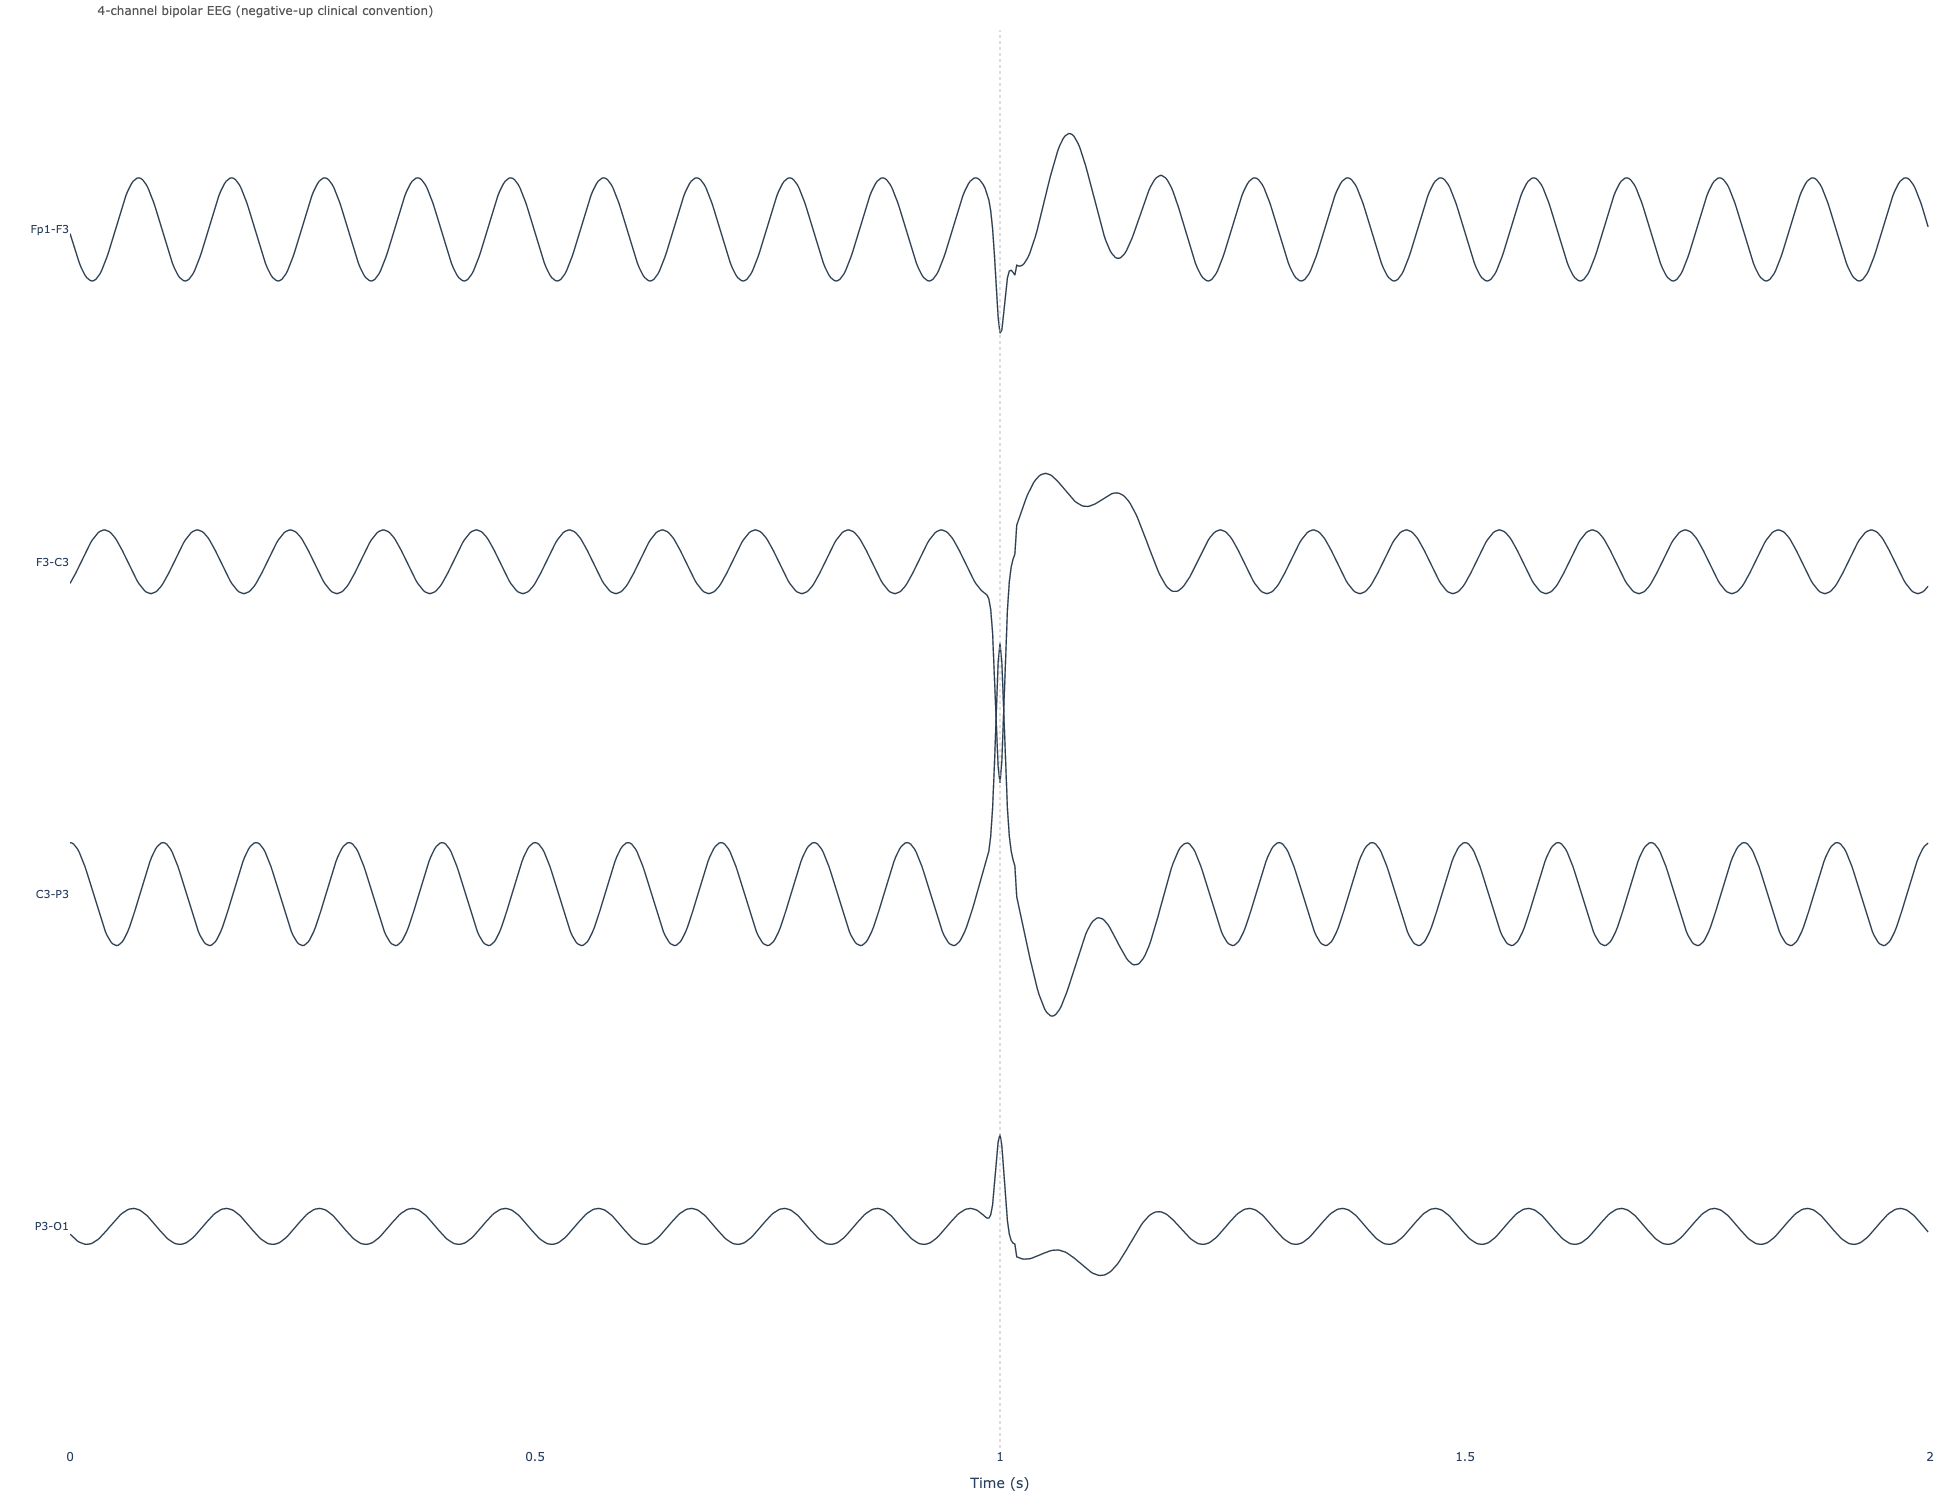
\includegraphics[width=0.95\textwidth]{figures/prob6_phase_reversal.png}
\end{center}

\begin{enumerate}[label=(\alph*),leftmargin=*]
\item Which electrode is closest to the spike source?
\item Explain in 2 sentences how you can tell.
\end{enumerate}

\vspace{4cm}
\hfill\textit{\small refer to: \href{https://judepj.github.io/neuro-signals-101/modules/05b_montages.html}{Module 5b — Montages}}

\vfill\pagebreak

% ──────────────────────────────────────────────────────────────────────
\section*{Problem 8 — The Double Banana}
The longitudinal bipolar montage (the ``double banana'') is the clinical
default for reading routine EEG.
\begin{enumerate}[label=(\alph*),leftmargin=*]
\item List the four electrode chains of the double banana, naming the electrodes in each chain in order from front to back.
\item All four chains run \textbf{front-to-back}. What kind of brain activity would this montage tend to underestimate, and why?
\end{enumerate}

\vspace{6cm}
\hfill\textit{\small refer to: \href{https://judepj.github.io/neuro-signals-101/modules/05b_montages.html}{Module 5b — The Double Banana Montage}}

\vfill\pagebreak

% ──────────────────────────────────────────────────────────────────────
\section*{Problem 9 — Artifacts}
The four panels below each show 3 seconds of EEG contaminated by a different
artifact. Identify the artifact in each panel (eye blink, muscle, 60\,Hz line
noise, ECG). For \textbf{one} of the four, give a one-sentence removal
strategy.

\begin{center}
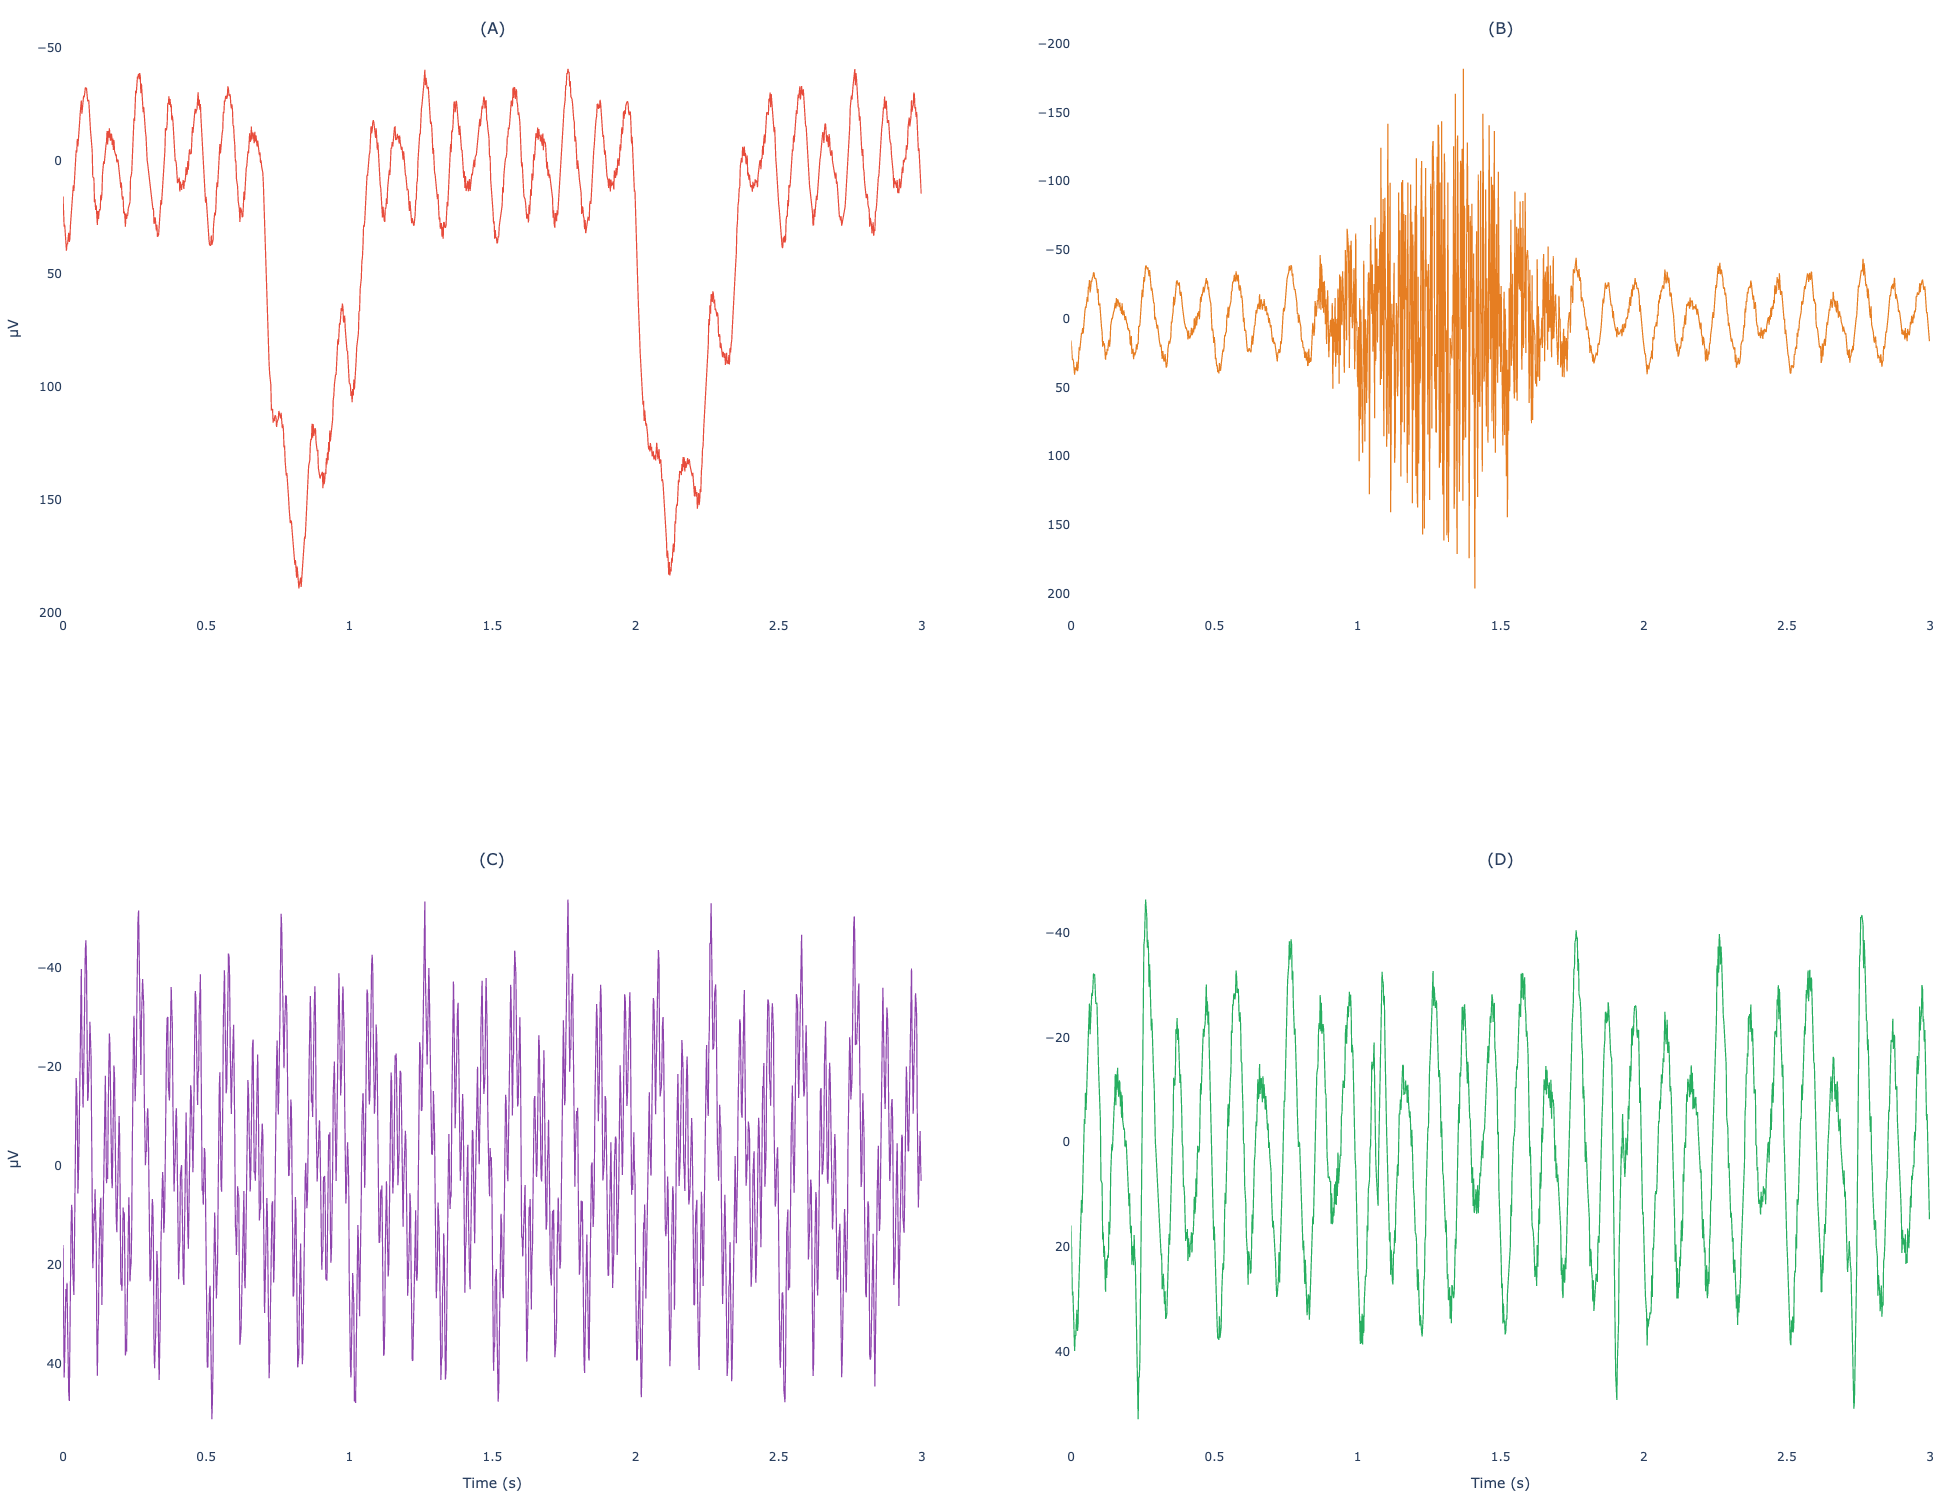
\includegraphics[width=0.95\textwidth]{figures/prob7_artifact_grid.png}
\end{center}

\begin{tabular}{p{2cm}p{12cm}}
\textbf{Panel} & \textbf{Artifact} \\
\hline
A & \\[0.8em]
B & \\[0.8em]
C & \\[0.8em]
D & \\[0.8em]
\hline
\end{tabular}

\vspace{0.6em}
\textbf{Removal strategy} (pick one panel):

\vspace{2.5cm}
\hfill\textit{\small refer to: \href{https://judepj.github.io/neuro-signals-101/modules/06_artifacts.html}{Module 6 — Artifacts}}

\vfill\pagebreak

% ──────────────────────────────────────────────────────────────────────
\section*{Problem 10 — Spectrograms}
Open the spectrogram widget in Module 7. Set the window length to
\textbf{0.5 seconds}, observe the spectrogram, then change it to
\textbf{2 seconds}.

\begin{enumerate}[label=(\alph*),leftmargin=*]
\item What improves and what gets worse when you go from 0.5\,s to 2\,s?
\item For detecting the precise moment a seizure begins on EEG, which window
would you choose? Why?
\end{enumerate}

\vspace{5cm}
\hfill\textit{\small refer to: \href{https://judepj.github.io/neuro-signals-101/modules/07_spectrograms.html}{Module 7 — Spectrograms}}

\vfill\pagebreak

% ──────────────────────────────────────────────────────────────────────
\section*{Problem 11 — The Real Thing (Module 8)}
Load the file \texttt{chb03\_01.edf} (provided with this tutorial, or download
from \href{https://physionet.org/content/chbmit/1.0.0/chb03/chb03_01.edf}{PhysioNet}).

\begin{enumerate}[label=(\alph*),leftmargin=*]
\item How many channels are in the recording? What is the sampling rate? How long is the recording in minutes?
\item What type of montage is this? (\textit{Hint: look at the channel names.})
\item Scroll through the recording. Something abnormal happens. At approximately what time (in seconds) does it start? How long does it last?
\item Compute a spectrogram for one channel around the abnormal event. Include the plot. Describe what you see in 1--2 sentences.
\item Based on the clinical vignette in Module 8 and your analysis: what is happening to this patient? Answer in 2--3 sentences.
\end{enumerate}

\vspace{5cm}
\hfill\textit{\small refer to: \href{https://judepj.github.io/neuro-signals-101/modules/08_challenge.html}{Module 8 — The Challenge}}

\end{document}
